\section{Обучаемые модели окружения}

\subsection{Планирование}

Понятно, что model-free алгоритмы, рассмотренные ранее, действуют не совсем так, как размышляет человек. Принимая решения, мы принимаем в учёт наши предсказания о том, в какое будущее выльется то или иное действие, и для построения предсказаний используем наши представления о том, как работает окружающий нас мир.

Итак, вернёмся к общей постановке задачи RL, и сейчас допустим, что нам доступен симулятор $p(s', r \mid s, a)$ для произвольных $s, a$ в произвольный момент времени.

В табличном сеттинге знание $p(s', r \mid s, a)$ позволяет применять алгоритмы динамического программирования Value Iteration и Policy Iteration. Однако, в табличном сеттинге мы умеем считать все интегралы --- мат.~ожидания по функции переходах; а в сложных средах знание функции переходов эти интегралы брать не позволяют.

Понятное дело, что, имея доступ к точному симулятору, мы можем, например, запустить какой-нибудь model-free алгоритм для обучения $\pi$, но нас интересует, можем ли мы непосредственно <<воспользоваться>> симулятором внутри самой стратегии, или даже придумать стратегию, использующую только симулятор. Раз мы полностью знаем правила игры, то, выбирая действие в некотором состоянии $s_0$, мы можем играть <<виртуальные>> игры, заглядывая в своё будущее. 

\begin{definition}
Для данного состояния $s_0$ набор действий $a_0, a_1, a_2, \dots$ будем называть \emph{планом} (plan).
\end{definition}

\needspace{5\baselineskip}
\begin{wrapfigure}{r}{0.4\textwidth}
\vspace{-0.5cm}
\centering
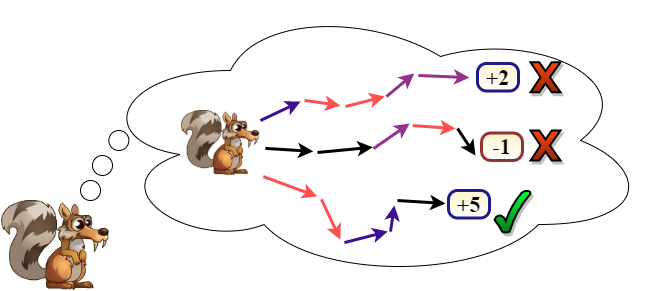
\includegraphics[width=0.4\textwidth]{Images/Planning.png}
\vspace{-0.5cm}
\end{wrapfigure}

Итак, допустим мы сидим в некотором $s_0$ и хотим найти хорошее действие $a_0$. Мы можем выбрать какое-нибудь $a_0$, засэмплировать $s_1$, выбрать как-то $a_1$, и так построить какой-нибудь план, для которого у нас будет сэмпл будущей награды. Можем так сделать, скажем, много раз. Нас ждёт две проблемы: у нас не получится рассмотреть всевозможные варианты будущего, и мы не сможем посчитать интеграл средней награды для одного плана; мы можем получить лишь сэмпл или Монте-Карло оценку по нескольким сэмплам.

\begin{example}
Какой типичный способ построения ИИ для ботов в играх: для текущего состояния $s$, в котором нужно выбрать действие, рассматривается несколько вариантов дальнейших действий на ближайшие шагов сто (при этом желательно заведомо неоптимальные варианты отсекать, чтобы сократить перебор); для каждого плана проводится симуляция (или несколько, если правила игры стохастичны и время позволяет). Играть до конца эпизода обычно дороговато, поэтому состояние $\hat{s}$, на котором симуляцию игры прервали, придётся оценивать при помощи какой-то эвристичной оценки $V^*(\hat{s})$.
\end{example}

Подобные алгоритмы могут <<спланировать>> свои будущие действия, а не выучить непосредственно зависимость $\pi(a \HM\mid s)$ (<<обучить стратегию>>).

\begin{definition}
Задача
\begin{equation}\label{planning}
\argmax_{a_0, a_1, a_2 \dots} \E_{\Traj \mid s_0, a_0, a_1, a_2 \dots} R(\Traj)
\end{equation}
при доступной функции переходов $p(s' \mid s, a)$ и функции награды называется \emph{планированием} (planning).
\end{definition}

В такой концепции понятия обучения нет. Для детерминированных MDP задача планирования по определению даёт оптимальный план, если задача \eqref{planning} решена точно, но для стохастичных MDP это неверно: 

\begin{theoremBox}[label=th:planningnotoptimal]{Неоптимальность планирования}
Пусть MDP стохастично и $a_0, a_1, a_2 \dots$ --- точное решение задачи \eqref{planning} для $s_0$. Тогда может быть такое, что для $a_0$ неоптимально ($Q^*(s_0, a_0) < Q^*(s_0, a)$ для некоторого $a \ne a_0$).

\needspace{5\baselineskip}
\begin{wrapfigure}{r}{0.3\textwidth}
%\vspace{-0.3cm}
\centering
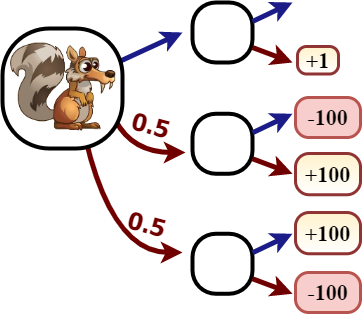
\includegraphics[width=0.3\textwidth]{Images/PlanningNonoptimal.png}
\vspace{-0.3cm}
\end{wrapfigure}
\beginproof
Посмотрим, чему равна средняя награда для каждого плана для MDP с рисунка. 

\begin{adjustwidth}{0.2\textwidth}{}
\begin{tabular}{cc}
План & Ценность плана \\
 \hline
(\colorsquare{ChadBlue}, \colorsquare{ChadRed})      & +1      \\ 
(\colorsquare{ChadBlue}, \colorsquare{ChadBlue})     & 0       \\
(\colorsquare{ChadRed}, \colorsquare{ChadRed})       & $\frac{1}{2}(+100 - 100) = 0$       \\
(\colorsquare{ChadRed}, \colorsquare{ChadBlue})      & $\frac{1}{2}(+100 - 100) = 0$       \\
\end{tabular}
\end{adjustwidth}

Значит, будет выбран <<безопасный>> вариант в виде плана (\colorsquare{ChadBlue}, \colorsquare{ChadRed}). Конечно же, оптимально выбрать в начале действие \colorsquare{ChadRed} и далее в зависимости от состояния выбрать то действие, которое даст +100, таким образом на самом деле $V^*(s_0) \HM= +100$.   \qed
\end{theoremBox}

% \begin{theorem}
% Пусть MDP стохастично и $a_0, a_1, a_2 \dots$ --- точное решение задачи \eqref{planning} для $s_0$. Тогда может быть такое, что для $s' \sim p(s' \mid s, a)$ план $a_1, a_2 \dots$ неоптимален.
% \begin{proof}
% Пусть в MDP из двух состояний и двух действий $r(s = 0, a = 0) \coloneqq \mathbb{I}[s = a]$ агент начинает в $s = 1$ и с вероятностью 0.9 остаётся в нём при любом действии. Тогда оптимальный план --- (1, 1, 1...), однако если агенту не повезёт и после выполнения оптимального действия $a_0 = 1$ среда закинет его в $s=0$, оптимальный план уже поменяется на (0, 0, 0...).
% \end{proof}
% \end{theorem}

Другими словами, планирование --- разумный подход в детерминированных средах, когда будущее предопределено. Поэтому большинство планировщиков, которые мы будем обсуждать далее, заточены именно под детерминированный случай. Важно, что даже в такой ситуации решать задачу \eqref{planning} точно, конечно же, не получится, и наше решение будет лишь приближённым. 

По этим двум причинам планировщик иметь смысл перезапускать на каждом шаге. Обычно алгоритм решения задачи планирования используется как просто <<очень вычислительно дорогая>> стратегия: сидя в $s_0$, алгоритм планирует совершить действия $a_0, a_1, a_2 \dots$; в реальной среде совершается лишь действие $a_0$, после чего для $s_1 \sim p(s_1 \mid s_0, a_0)$ алгоритм планирования запускается ещё раз (важно, что тут он может использовать какую-то информацию с прошлого процесса планирования) для определения $a_1$ и так далее. Так важно делать в том числе потому, что в реальности точное решение \eqref{planning} мы не получим, и вместо него может быть лишь приближённое решение. Планировщик, в частности, может понимать, что он не рассмотрел всевозможные исходы будущего, и из этих соображений выдать вероятностное распределение $\pi(a_0 \HM\mid s_0)$; тогда стратегия, полученная при помощи такого планировщика, будет стохастична.

\begin{example}[Мета-эвристики как планировщики]
Для решения \eqref{planning} можно использовать, например, случайный поиск. Сидя в $s_0$, засэмплируем 100 случайных планов и при помощи симулятора посчитаем для каждого из них сэмплы $R(\Traj)$; выберем то $a_0$, для которого нашлась траектория с максимальным сэмплом reward-to-go. Если среда детерминирована, то $a_0$ гарантировано позволяет получить такую награду; что не означает, что мы нашли наилучший план, и оптимальным может оказаться другое действие. Если среда стохастична, то даже гарантий получить <<найденный>> reward-to-go нет, поскольку это лишь сэмпл и нам могло в симуляции просто повезти. Выбранное $a_0$ отправляется в среду; для сэмпла $s_1$ из реальной среды процесс планирования запускается заново. 

%Какими-нибудь эвристиками можно учесть результаты с прошлой итерации планирования; например, если во время планирования из $s_0$ у нас были планы, в которых в симуляциях встречалось $s_1$, мы можем переиспользовать эти сэмплы.

%TODO: CEM as planning?
\end{example}

То есть, обучения в такой концепции нет, но каждое принятие решения алгоритмом (каждый <<запуск стратегии>>) --- это целый процесс оптимизации, что обычно очень дорого.

\subsection{Модели мира (World Models)}

В реальной жизни в рамках нашей общей постановки задачи функция переходов и награды $p(s', r \mid s, a)$ нам неизвестна. Тем не менее, у нас есть опция как-то попытаться её выучить и как-то использовать для улучшения наших алгоритмов. Открывается два вопроса: как учить и как использовать.

\begin{definition}
\emph{Моделью мира} (world model) называется любая модель, явно или неявно обучающаяся модели динамики среды.
\end{definition}

Под <<явно или неявно>> подразумевается, что это не обязательно должна быть функция, по состоянию и действию возвращающая следующее состояние, хотя, конечно, это самая стандартная опция.

\begin{remark}
Модель мира также может сжимать описание состояний в некоторое латентное пространство, которое далее может использовать стратегия. Ещё можно нарушить end-to-end парадигму и в целом отдельно выучить автокодировщик, который сожмёт описание состояний в некоторый компактный векторочек; RL же применять только для обучения самой стратегии, которая будет принимать на вход такое компактное описание состояний. \href{https://worldmodels.github.io/assets/mp4/carracing_vae_compare.mp4}{Пример подобного сжатия}.
\end{remark}

Простейший способ <<использовать>> выученную модель --- взять в качестве стратегии какой-нибудь планировщик, который будет работать с обученной аппроксимацией модели мира будто это истинная модель. Нюанс такого подхода заключается в том, что планировщик по определению <<хорош>> только если модель мира точна. Если модель мира обучается только на тех примерах, которые мы встречаем в нашем опыте, то мы рискуем познать только тот мир, который обозревает наша текущая стратегия. До <<генеральной совокупности>> подобному опыту может быть далеко, и поэтому необходимо постоянно дообучать модель мира после каждого улучшения стратегии.

\begin{algorithm}{Общая схема Model-based подхода}
\textbf{Гиперпараметры:} Планировщик, модель мира.

\vspace{0.3cm}
Проинициализировать стратегию $\pi_0(a \mid s)$ случайно. \\
Проинициализировать модель мира случайно. \\
Проинициализировать датасет пустым множеством. \\
\textbf{На $k$-ом шаге:}
\begin{enumerate}
    \item Повзаимодействовать со средой при помощи $\pi_k$, добавив встреченные переходы $\{s, a, r, s'\}$ в датасет.
    \item Провести дообучение модели мира на собранном датасете:
    \item Получить $\pi_k$ из планировщика, используя текущую модель мира.
\end{enumerate}
\end{algorithm}

Под словами <<получить $\pi_k$ из планировщика>> здесь понимается, что далее в качестве стратегии $\pi_k$ используется запуск планировщика, который кушает текущее состояние, рассматривает какие-то планы и выдаёт первое действие наилучшего плана $a_0$ или какое-то распределение в пространстве действий, <<вероятности того, что $a_0$ соответствует оптимальному плану>>.

\subsection{Модель прямой динамики}

\begin{definition}
Модель функции переходов $p_\theta(s' \mid s, a)$ называется \emph{моделью прямой динамики} (forward dynamics model).
\end{definition}

\needspace{5\baselineskip}
\begin{wrapfigure}{r}{0.6\textwidth}
\vspace{-0.5cm}
\centering
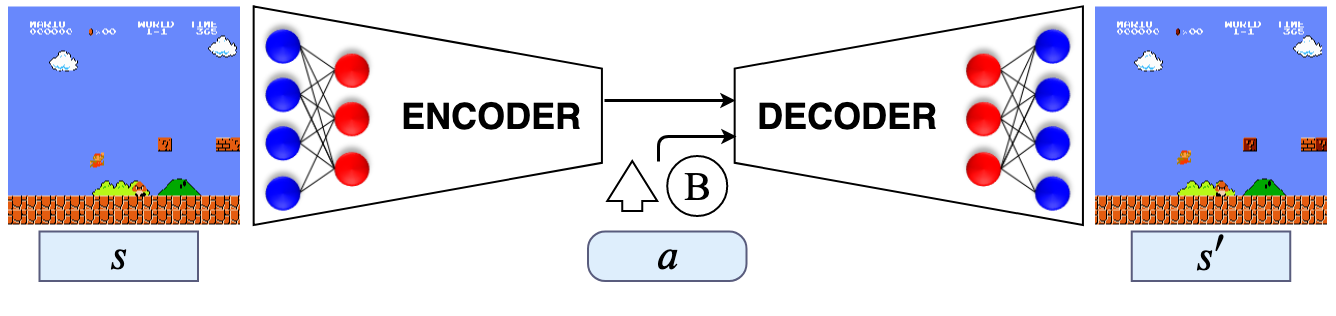
\includegraphics[width=0.6\textwidth]{Images/MarioVAE.png}
\vspace{-0.5cm}
\end{wrapfigure}

Учить генеративную модель может быть дороговато, и простым удешевлением является обучение детерминированного приближения $s' \approx f_\theta(s, a)$. Это можно делать по любым доступным траекториям, собранным любым способом:
$$\sum_{s, a, s'} \|f_\theta(s, a) - s'\|^2 \to \min_\theta$$
$$\sum_{s, a, r} \left( r_\psi(s, a) - r \right)^2 \to \min_\psi$$

Этот лобовой подход многим плох. В сложных средах описание состояний обычно содержит огромное количество никак не связанной с задачами агента информацией; например, декоративные элементы в видеоиграх. Обучение подобной $f_\theta$ сопряжено с бессмысленным изучением этой информации. Наконец, если состояния $s$ --- картинки, то в текущей формуле сгенерированное изображение сравнивается с реальным $s'$ по l2-метрике; для изображений это не сильно осмысленно, конечно, и нужно придумывать что-то другое.

%TODO: картинки

\begin{remark}
Иногда в задачах робототехники можно в модель прямой динамики внести <<inductive bias>>, используя знания о том, что модель динамики представляет собой какое-то дифференциальное уравнение. Тогда могут искаться параметры функций, стоящих внутри уравнений связи, а в качестве итоговой модели использоваться какая-то дискретизация <<обученного>> диффура.
\end{remark}

\subsection{Сновидения}

Наличие модели прямой динамики $p_\theta(s', r \mid s, a)$ позволяет нам при помощи текущей стратегии $\pi$ генерировать траектории, используя полностью наши <<внутренние модели>> и никак не используя реальную внешнюю среду. Это означает, что в случае обучаемой модели динамики мы теоретически можем начать симулировать опыт при помощи, условно, нашей генеративной модели, и обучать на нём model-free алгоритм.

\begin{definition}
\emph{Сновидениями} (dreaming) называется обучение агента на опыте, собранном при помощи приближения динамики среды $p_\theta(s', r \mid s, a)$.
\end{definition}

Далеко мы так, конечно, не уедем, поскольку наша генеративная модель вряд ли будет идеальна: регулярно нужно <<просыпаться>> и отправляться в реальную среду собирать сэмплы для улучшения как минимум модели мира. Тем не менее, использование снов может существенно повысить sample efficiency алгоритмов: потребуется меньше реальных взаимодействий со средой, и большую часть процесса обучения самой стратегии можно переложить на сны. Цена --- в вычислительной неэффективности: траекторий во сне из-за отличий от реальных потребуется генерировать довольно много. То есть, хотя шагов взаимодействия с настоящей средой станет меньше, время обучения алгоритма (wall-clock time) наоборот увеличится. 

%TODO: пример

\begin{remark}
В целом, любой model-based подход в обучении с подкреплением обычно позволяет выиграть именно в терминах sample efficiency за счёт долгих вычислений, за счёт увеличения wall-clock time. Полностью противоположная ситуация у нас была в мета-эвристиках (глава \ref{metaheuristicchapter}): там наоборот за счёт огромного числа сэмплов можно было обучить алгоритм достаточно быстро (при наличии ресурсов параллелизации). Классические model-free алгоритмы на основе Value-based и Policy Gradient подхода при этом находятся где-то в хорошей середине, и если ресурсов параллелизации нет, а взаимодействие со средой не является катастрофически дорогим, они обычно оказываются в выигрыше.
\end{remark}